\documentclass[a4paper]{report}

\usepackage[american]{babel}
\usepackage[latin1]{inputenc}
\usepackage{amsmath}
\usepackage{amsfonts}
\usepackage{hyperref}
\usepackage{xspace}
\usepackage{textcomp}
\usepackage{tabularx}
\usepackage{alltt}
\usepackage{url}
\usepackage{vaucanson-g}
\usepackage{graphicx}
\usepackage{tabularx}
\usepackage{texi}

\usepackage{listings}
\lstset{%
  numbers=left,
  numberstyle=\tiny,
  stepnumber=5,
  numbersep=5pt,
  firstnumber=1,
  basicstyle=\small,
  frame=single,
  language=C++,
  float}

\newenvironment{cmp}{%
  \begin{center}
    \begin{minipage}{\textwidth}}{%
    \end{minipage}
  \end{center}}

\newcommand{\textrp}[1]{\textit{#1}}
\newcommand{\textarg}[1]{\textsl{#1}}
\newcommand\inputcode[4][]{%
  \begin{figure}[htbp]
    \centering
    \begin{minipage}{0.9\textwidth}
      \lstinputlisting[language=C++, #1]{#2}
    \end{minipage}
    \caption{#3}
    \label{fig:#4}
  \end{figure}}

\usepackage{graphicx}
\graphicspath{{figures/}}

\newcommand{\Vauc}{\textsc{Vaucanson}\xspace}

\title{\Vauc User's manual}
\author{The \Vauc group}
\setcounter{tocdepth}{2}

\makeindex

\begin{document}

\maketitle

\tableofcontents

\chapter{Installation}

\section{Getting \Vauc}

The latest stable version of the \Vauc platform can be downloaded
from \url{http://vaucanson.lrde.epita.fr/}.  The current development
version can be retrieved from its Subversion\footnote{%
%%
  Subversion can be found at \url{http://subversion.tigris.org/}.
%%
} repository as follows:

\begin{shell}
# \kbd{svn checkout https://svn.lrde.epita.fr/svn/vaucanson/trunk vaucanson}
\end{shell}

\section{Building \Vauc}

The following commands build and install the platform:
\begin{shell}
# \kbd{cd vaucanson-\VcsnVersion}
\end{shell}
Then:
\begin{shell}
# \kbd{./configure}
...
# \kbd{make}
...
# \kbd{sudo make install}
...
\end{shell}

More detailed information is provided in the files \file{INSTALL},
which is generic to all packages using the GNU Build System, and
\file{README} which details \Vauc's specific build process.

%%% Local Variables:
%%% mode: latex
%%% ispell-local-dictionary: "american"
%%% TeX-master: "vaucanson-user-manual"
%%% End:

% LocalWords:  svn vaucanson cd sudo

\chapter{\Vauc as a toolkit}

\Vauc provides several programs that manipulate various type of
automata. In this chapter we will learn
how to use those programs. Actually there are 6 programs
located in src/demos/function\_library/ directory. Each of them
dealing with a specific type of automata:

\begin{itemize}
  \item b for manipulating automata over Boolean semiring $\mathbb{B}$;
  \item z for manipulating automata over $(\mathbb{Z},+)$;
  \item z\_min\_plus for manipulating automata over $(\mathbb{Z},min)$;
  \item z\_max\_plus for manipulating automata over $(\mathbb{Z},max)$;
  \item rt\_tdc for manipulating realtime transducers;
  \item tdc for manipulating automata over free monoid product.
\end{itemize}

The first step before starting to work with \Vauc toolkit is to choose
on which type of automata you intend to work. Then you should just use
the proper program between those listed before.

%%Example on boolean automaton
\section{Boolean automata}

This part show the use of the program \textit{b}.

\subsection{A first example}

%%FIXME: Ref marche pas
Let's consider the following boolean automaton \ref{A_1} :

%%Schema de l'automate A1
\begin{figure}[ht] \centering
  \begin{VCPicture}{(0,-2)(6,2)}
    % states
    \State{(0,0)}{A} \State{(3,0)}{B} \State{(6,0)}{C}
    % initial--final
    \Initial{A} \Final{C}
    % transitions
    \EdgeL{A}{B}{a} \EdgeL{B}{C}{b}
    \LoopS[.5]{A}{b} \LoopN[.5]{A}{a} \LoopS[.5]{C}{b} \LoopN[.5]{C}{a}
    %
  \end{VCPicture}
  \caption{The automaton $A_1$}
  \label{A_1}
\end{figure}

You can find the XML code that describe this automaton in
doc/manual/examples/a1.xml.
We will use \Vauc to compute the determinized automaton of $A_1$ and
then we will minimize the resulting automaton.

\subsubsection{Determinization of $A_1$}
Computing the determinized of a boolean automaton is simply realized
by calling \textit{determinize} function :
\begin{alltt}
# ./b determinize a1.xml > a1\_det.xml
\end{alltt}
Now the file a1\_det.xml contains the XML description of the
determinized of the automaton A.

\subsubsection{Visualizing}

We can get some information about our newly created automaton by calling
the \textit{info} function:
\begin{alltt}
# ./b info a1\_det.xml
\textit{States: 4
Transitions: 8
Initial states: 1
Final states: 2}
\end{alltt}
Or we can use dotty to visualize our newly created automaton:
\begin{alltt}
# ./b display a1\_det.xml
\end{alltt}

%%Dotty output of det(A1)
%%\begin{figure}[ht]
\begin{center}
  \scalebox{0.7}{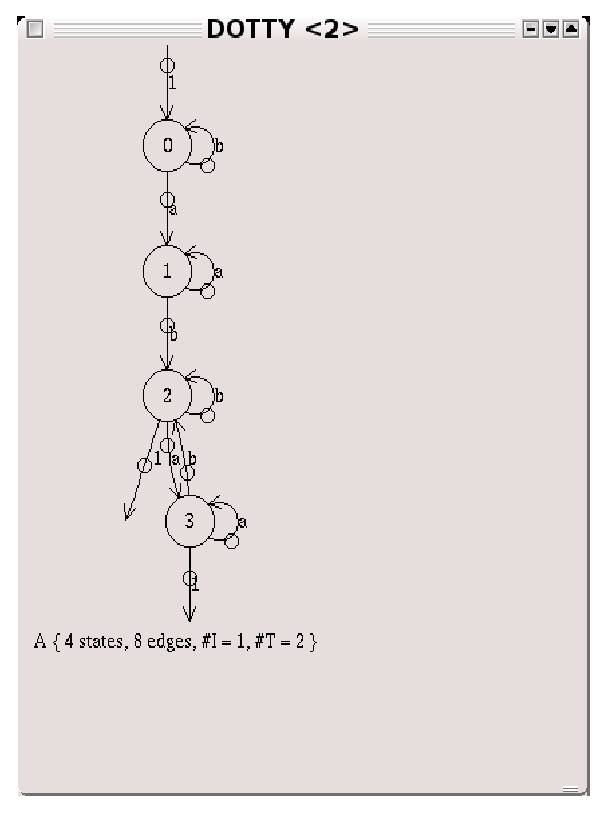
\includegraphics{images/a1_det.eps}}
\end{center}
%%  \caption{Determinized of $A_1$}
%%\end{figure}

\subsubsection{Minimizing}

\begin{alltt}
# ./b determinize a1.xml | ./b minimize - | ./b display -
\end{alltt}

%% Dotty min(det(A1))
%%\begin{figure}[!h]
\begin{center}
  \scalebox{0.7}{\includegraphics{images/a1_det_min.eps}}
\end{center}
%%\caption{Minimizing the Determinized of $A_1$}
%%\end{figure}

\subsubsection{Evaluation}

Evaluating if a word is accepted by our automaton :
\begin{alltt}
# ./b eval a1.xml 'abab'
\textit{1}
# ./b eval a1.xml 'bbba'
\textit{0}
\end{alltt}
where 1 (resp. 0) means that the word is accepted (resp. not accepted)
by the automaton.

\subsection{Rationnal expressions and boolean automata}

\Vauc provides functions for manipulating rationnal expressions
associated to boolean automata. For instance, computing the language
recognized by a boolean automaton can be done thanks to the
\textit{aut\_to\_exp} function:
\begin{alltt}
# ./b aut_to_exp a1.xml
\textit{(a+b)*.a.b.(a+b)*}
# ./b aut_to_exp a1_det.xml
\textit{b*.a.a*.b.(a.a*.b+b)*.(a.a*+1)}
\end{alltt}
Plus \Vauc provides several algorithms that build an automaton that
recognizes a given language. For instance let's build the standard
automaton that recognizes the language "$(a+b)*a.b.(a+b)*$" and
minimize the resulting automaton:

\begin{alltt}
# /b standard_of "(a+b)*a.b.(a+b)*" | ./b minimize - | ./b display -
\end{alltt}
%%\begin{figure}[ht]
\begin{center}
  \scalebox{0.7}{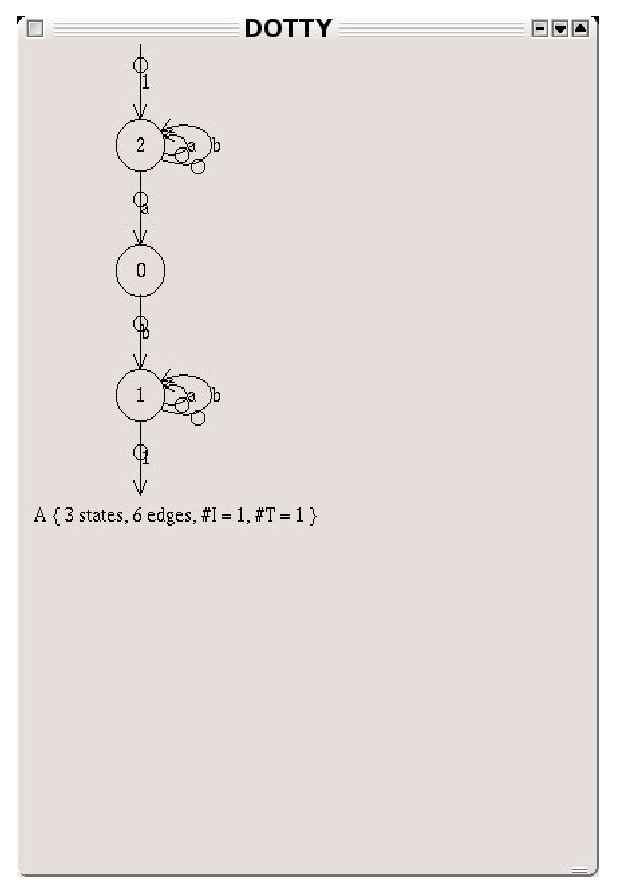
\includegraphics{images/a1.eps}}
\end{center}
%%  \caption{The minimize standard automaton of "(a+b)*a.b.(a+b)*"}
%%\end{figure}
Please note that your rationnal expressions should follow the
following grammar. %%Fixme : Lien vers la grammaire des ratexp
%% \begin{verbatim}
%%         exp ::= '(' exp ')'
%%         |   exp '+' exp
%%         |   exp '.' exp
%%         |   exp exp
%%         |   exp '*'
%%         |   weight ' ' exp
%%         |   exp ' ' weight
%%         |   0
%%         |   1
%%         |   word
%% \end{verbatim}

\subsection{Description of available funtions}
%% Fixme: A finir
%%
%% Une definition plus rigoureuse des algorithmes devrait etre fournie
%% en annexe.
In this section you will find a brief definition of all functions that
\Vauc provides for manipulating boolean automata.\\
\begin{itemize}
\item[-] \textit{a1.xml} \textit{a2.xml} are two boolean automata described in
  \Vauc XML format.
\item[-] \textit{w} is a word, for example \textit{"aabb"} if you are working on an
  alphabet that contains the letters \textit{a} and \textit{b}.
\item[-] \textit{exp} is a rationnal expression denoting a language.
\item[-] \textit{n} is a strictly positive integer.
\end{itemize}

\begin{description}
  \item [are-isomorphic] :\\
    ./b a1.xml a2.xml\\
    Return 1 (resp. 0) if the two automata are (resp. aren't)
    isomorphic.

  \item [aut\_to\_exp] : \\
    ./b aut\_to\_exp a1.xml\\
    Return a regular expression denoting the langage recognized by
    \textit{aut}.

  \item [accessible] :\\
    ./b accessible a1.xml\\
    Extract the sub-automaton of accessible states of a1.xml.

  \item [closure] :\\
    ./b closure a1.xml\\
    Complete the automaton a1.xml to make it
    close over epsilon transition (based on the
    Floyd-McNaughton-Yamada algorithm).

  \item [co-accessible] :\\
    ./b accessible a1.xml\\
    Extract the sub-automaton of co-accessible states of a1.xml.

  \item [derived\_terms] :\\

  \item [determinize] :\\
    ./b determinize a1.xml\\
    Return the determinized of a1.xml.

  \item [display] :\\
    ./b display a1.xml\\
    Display a graphical view of the automaton a1.xml using DOT format.

  \item [evaluation] :\\
    ./b eval a1.xml w\\
    Return 1 (resp. 0) if the word w is accepted by the automaton
    a1.xml

  \item [expand] :\\

  \item [info] :\\
    ./b info a1.xml\\
    Display general information (Number of states, number of
    transitions, number of initial states and number of final
    states) on the automaton \textit{a1.xml}.

  \item [is-empty] :\\
    ./b is-empty a1.xml\\
    Return 1 (resp. 0) if the automaton has (resp. hasn't) accessible
    or (resp. and) co-accessible states.

  \item [minimize] :\\
    ./b minimize [hm] a1.xml\\
    Return the minimal automaton of a1.xml (By default the minimal
    automaton is built using Hopcroft algorithm).
    \begin{itemize}
      \item[-] h Use Hopcroft algorithm
      \item[-] m Use Moore algorithm
    \end{itemize}

  \item [power] :\\
    ./b power a1.xml n\\
    Return the ...

  \item [product] :\\
    ./b product a1.xml a2.xml\\
    Return the product of the two automata.

  \item [quotient] :\\
    ./b quotient a1.xml\\
    Return the quotient of a non deterministic automaton.

  \item [realtime] :\\
    ./b realtime a1.xml\\
    Return the realtime automaton of the automaton a1.xml.

  \item [standard\_of] :\\
    ./b standard\_of exp\\
    Return the standard automaton build from the rationnal expression exp.

  \item [trim] :\\
    ./b trim a1.xml\\
    Return the trimmed automaton of a1.xml.

  \item [transpose] :\\
    ./b transpose a1.xml\\
    Return the transposed of the automaton a1.xml.

  \item [thompson\_of] :\\

\end{description}

\section{Transducers}
%%FIXME: L'algorithme fmp_to_trans et trans_to_fmp devrait paut-etre fournit par
%%ces programmes.
\subsection{Example}

The transducer $T$(\ref{bindiv3}) gives the quotient by 3 of a binary number.

\begin{figure}[h]
  \begin{center}
    \begin{VCPicture}{(0,-2)(6,2)}
% states
\State{(0,0)}{A} \State{(3,0)}{B} \State{(6,0)}{C}
\Initial[w]{A}
\Final[s]{A}
%transitions
\LoopN{A}{\IOL{0}{0}}
\LoopN{C}{\IOL{1}{1}}
\ArcL{A}{B}{\IOL{1}{0}}
\ArcL{B}{A}{\IOL{1}{1}}
\ArcL{B}{C}{\IOL{0}{0}}
\ArcL{C}{B}{\IOL{0}{1}}
\end{VCPicture}
\caption{Transducer $T$ giving the quotient by 3 of a binary number}
\label{bindiv3}
  \end{center}
\end{figure}

\subsubsection{Evalutation}


\section{Weighted automata}

This part shows the use of the program \textit{z}, (but all
comments should also stand for the programs \textit{z\_min\_plus and
z\_max\_plus}).

\subsection{Example}

Let's consider the following $\mathbb{N}$-automaton, \textit{i.e.}
an automaton which label's weights are in $\mathbb{N}$:

%%Schema de l'automate B1
\begin{figure}[ht] \centering
  \begin{VCPicture}{(0,-2)(3,2)}
    % states
    \State{(0,0)}{A} \State{(3,0)}{B}
    % initial--final
    \Initial{A} \Final{B}
    % transitions
    \EdgeL{A}{B}{b}
    \LoopS[.5]{A}{b} \LoopN[.5]{A}{a}
    \LoopS[.5]{B}{b} \LoopN[.5]{B}{a}
    %
  \end{VCPicture}
  \caption{The automaton $B_1$}
\end{figure}

This time the evaluation of the word \textit{w} by the automaton $B_1$
will produce a number, rather than simply accept or reject \textit{w}.
For instance let's evaluate "abab" and "bbab":

\subsubsection{Evaluation}

\begin{alltt}
# ./z eval b1.xml 'abbb'
\textit{3}
# ./z eval b1.xml 'abab'
\textit{2}
\end{alltt}

As you may have already guessed the automaton $B_1$ "counts" the
number of 'b' contained in \textit{w}.

\subsubsection{Power}

Now let's consider the $B_1^4$, where
$$B_1^4 = \prod_{i=1}^4 B_1, 4 > 0$$

\begin{alltt}
# ./z eval b1.xml 4 > b1_4.xml
\end{alltt}

Now the file \textit{b1\_4.xml} contains the automaton $B_1^4$. Lets
see what the evaluation of the words "abab" and "bbab" gives with this
automaton:

\begin{alltt}
#./z eval b1_4.xml 'bbab'
\textit{81}
./z eval b1_4.xml 'abab'
\textit{16}
\end{alltt}

This time one can notice that the automaton $B_1^4$ returns the
evaluation of $B_1$ but at power 4.

\subsection{Description of available funtions}


\section{Building your own automaton}
%%FIXME: Here we should give the usage of define_automaton function.

\chapter{\Vauc as a library}


\end{document}